\section{関連研究}
\label{sec:related-works}
本章では,次世代DNSとして提案されている名前解決システムを紹介し,DNSトンネリングへの抑止効果を焦点に提案システムとの違いを説明する.
%先行研究のシステムは,以下に示す2つに分類できる.
%\begin{description}
% \item[P2Pネットワーク]\mbox{}\\ ノードとコンテンツに同一識別子を付与し,対象のコンテンツに近いノードを再帰的に問い合わせることによってコンテンツ情報を取得するシステム. \\(手法例) : DDNS, HDNS, GNU
% \item[中央集権]\mbox{}\\ 中央集権的なサービスもしくはノードに問い合わせることで解決するシステム.\\(手法例) : 初期システム,Namecoin, Blockname, Blockstack
%\end{description}

\subsection{P2Pネットワーク}
本節では,P2Pネットワークに基づいたDNSについて説明する.
クライアントとサーバを排除し,ノード間をピアで接続するP2Pネットワークには耐障害性とスケーラビリティの特性がある.
この優位性を名前解決に応用した手法は,過去に複数提案されている.
Coxら~\cite{cox}は,既存システムの管理における非効率なロードバランシングと低い障害耐性の課題を解決することを目的にP2Pネットワークに基づいたシステムを提案している.
提案されたシステムDDNS(Distributed domain name system)は,既存システムの再帰問い合わせの仕組みに代わる,Chordアルゴリズムを使ったDHashに基づいてサーバ探索することで目的を実現させる~\cite{dhash}.
システムにおける名前解決の仕組みは,図~\ref{fig:chord}で示すように,ハッシュ関数によって算出されたIDに基づいてノードとコンテンツをリング状に射影し,コンテンツに近いノードがコンテンツ情報を管理・応答することによって機能する.
\begin{figure}[bhtp]
 \centering
 \label{fig:chord}
 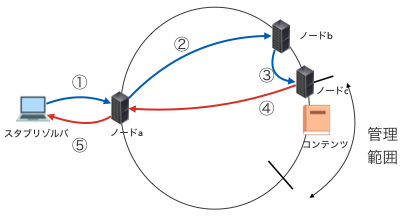
\includegraphics[scale=0.6]{figure/chord-mechanism.png}
 \caption{DDNSにおける名前解決プロセス}
\end{figure}
クライアントからの問い合わせを受け取ったノードaは,クエリされたコンテンツIDを導出し,経路情報に明記されたIDのリストの内で最も近しいノードbにクエリを転送する.
コンテンツのIDに最も近いノードcまで再帰的に問い合わせられると,最終的にコンテンツを保持するノードcがコンテンツ情報をノードaに応答することで名前が解決される.
Chordリング上では,コンテンツIDと経路情報に基づいて宛先ノードが決まるため,特定ノードにデータを意図的に転送することは難しく,DNSトンネリングの発生を抑止することできる.
しかし,Chordアルゴリズムではコンテンツを保持するノードの探索が非効率であることが指摘されている.
線型探索の課題を改善するために,``finger table"に基づいていくつかのノードをスキップ手法が提案されているが,この場合の探索でも$O(\log N)$のクエリを必要とするため,パフォーマンスの課題がある~\cite{p_donas}.

Yitingら~\cite{yiting}は,P2Pネットワークにおける遅延の課題を解消するHDNS(hybrid DNS)を提案している.
提案システムは,Public Zoneと呼ばれるChordアルゴリズムに基づいたP2Pネットワークと,Internal Zoneと呼ばれる従来の階層型DNSツリー構造を組み合わせで構成されている.
図~\ref{fig:hdns-mechanism}で示すように,クエリはDDNS同様の要領でコンテンツに近いノードに転送した後,階層構造に基づきクエリを転送する.
HDNSでは,パフォーマンスこそ改善されるが,コンテンツを保持するノードがドメイン名の階層構造に従うため,DNSトンネリンを抑止することはできない.
\begin{figure}[htbp]
 \centering
 \label{fig:hdns-mechanism}
 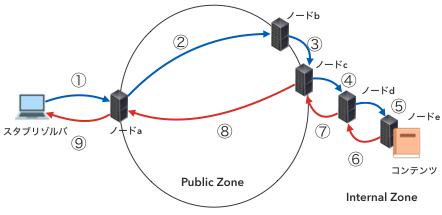
\includegraphics[scale=0.6]{figure/hdns-mechanism.png}
 \caption{HDNSにおける名前解決プロセス}
\end{figure}

GNU~\cite{gns}は,DNSにおけるプライバシーの課題を解消することを目的に,ピュアなP2Pで接続するGNSを提案している.
GNSでは,全てのユーザが自身の名前空間を保持・管理し(例: .bob),また他のユーザにサブドメインを委譲できる(例: .sample.bob)設計になっている.
図~\ref{fig:gns-resolution}は,Aliceリゾルバが``www.bob.dave.gun"と``www.carol.dave.gnu"という名前を解決するために辿るパスを示している.
このように,ユーザ間はピュアなP2Pで接続され,更に通信には暗号化を前提としているという特徴がある.
GNSでは,擬似的なTLDとして``.gnu"が使われるなど,従来の名前空間とは全く異なる.
GNSでは,ユーザ同士が暗号化した通信を用いて直接やりとりため,既存システムにおけるDNSトンネリングの仕組みでデータを転送することを許す設計になっている.
\begin{figure}[htbp]
 \centering
 \label{fig:gns-resolution}
 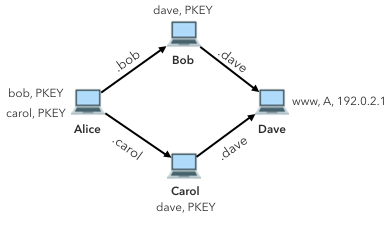
\includegraphics[scale=0.6]{figure/gns-resolution.png}
 \caption{GNSにおける名前解決プロセス}
\end{figure}

\subsection{課題}
\label{sec:issue-past-works}
上記で説明してきたように,同一のハッシュ関数から導出されるIDを持つコンテンツとノードをP2Pネットワークに構築する手法だけが,DNSトンネリングを抑止することができる.
しかし,この手法に基づいた名前解決では,既存システムと比べて大きな遅延が発生するという課題がある.
その他に提案されてきたシステムでは,DNSトンネリングの手法は依然として利用できてしまう.
次章では,DNSトンネリング抑止機能だけでなく,高速な名前解決の両方を備える提案システムについて説明する.

%\subsection{中央集権}
% 初期システム
% Namecoin
% Blockname
% Blockstack
% 提案手法
